% This file is iccc.tex.  It contains the formatting instructions for and acts as a template for submissions to ICCC.  It borrows liberally from the AAAI and IJCAI formats and instructions.  It uses the files iccc.sty, iccc.bst and iccc.bib, the first two of which also borrow liberally from the same sources.

\documentclass[letterpaper]{article}
\usepackage{iccc}
\usepackage{graphicx}

\usepackage{times}
\usepackage{helvet}
\usepackage{courier}

\graphicspath{ {images/} }

\pdfinfo{
/Title (Human-Level Concept Learning for Musical Metacreativity in Lyrical Sectional-Form Symbolic Music)
/Subject (Doctoral Consortium at ICCC 2017)
/Author (Paul Bodily)}
% The file iccc.sty is the style file for ICCC proceedings.
%
\title{Human-Level Concept Learning for Musical Metacreativity in \\Lyrical Sectional-Form Symbolic Music}
\author{Paul Bodily\\
Computer Science Department\\
Brigham Young University\\
Provo, UT 84602  USA\\
paulmbodily@gmail.com\\
}
\setcounter{secnumdepth}{0}

\begin{document} 
\maketitle
\begin{abstract}
\begin{quote}
We present a human-level concept learning model for generating lyrical, sectional-form, symbolic lead sheets. This approach involves decomposing a model of lyrical composition into several constituent subconcept models. Approximating subconcepts is simpler than directly approximating the aggregate concept and facilitates independence assumptions that lead to a wider range of expression. Two principle challenges exist to this approach. First is determining how the aggregate model should be factored to enable effective learning. Second is deriving means of accurately approximating subconcept models. Our research focuses on precisely defining these challenges to facilitate community dialogue and presenting solutions to these problems to demonstrate the effectiveness of the concept-learning approach.
\end{quote}
\end{abstract}

\section{Introduction}
Common in the field of computational creativity is the argument that \emph{computers} can exhibit creativity without directly imitating the process by which \emph{humans} exhibit creativity. Independent of this debate, it is valuable to consider the process by which humans are creative, particularly given that, in terms of producing novel, interesting, and valuable artefacts, humans are the most creative entities in the known universe.

One of the hallmark characteristics of human creativity and intelligence is that of human-level concept learning. Human-level concept learning is the idea that concepts are decomposed into simpler subconcepts and that the original concept can be learned by thoroughly learning each of the subconcepts (i.e., \emph{learning-to-learn}). For example, when learning to play an accordion, a human would likely decompose the accordion into subparts (e.g., keyboard, bellows, bass buttons) and then learn (or apply previous learning of) each of these subparts individually (see Figure~\ref{fig:accordion}). This process has been shown to be extremely effective in one-shot classification, parsing, and generation of hand-written characters \cite{lake2015human}.

The fundamental question that drives our research is: \emph{how might human-level concept learning be applied to effectively model concepts in computational creativity}? As a concrete domain for our exploration of this topic we focus specifically on lyrical, sectional-form, symbolic lead sheets.

Much prior work relates to generating lyrical lead sheets, including research on assisted lead sheet composition \cite{papadopoulos2016assisted}; composition of art songs \cite{toivanen2013automatical}; composing music for lyrics \cite{scirea2015smug,monteith2012automatic}; and generation of lyrics both with \cite{ramakrishnan2009automatic} and without a pre-existing melody \cite{gonccalo2015tra}. However, none of these studies directly address sectional-form music and most do not consider joint composition of all view points of lyrical music.

In what follows we define a mathematical model of human-level concept learning in pop music composition; establish data-driven methods for (abstract) subconcept learning; and discuss improving model definitions and model approximations via artistic intuition.

\begin{figure}[th]
	\centering
	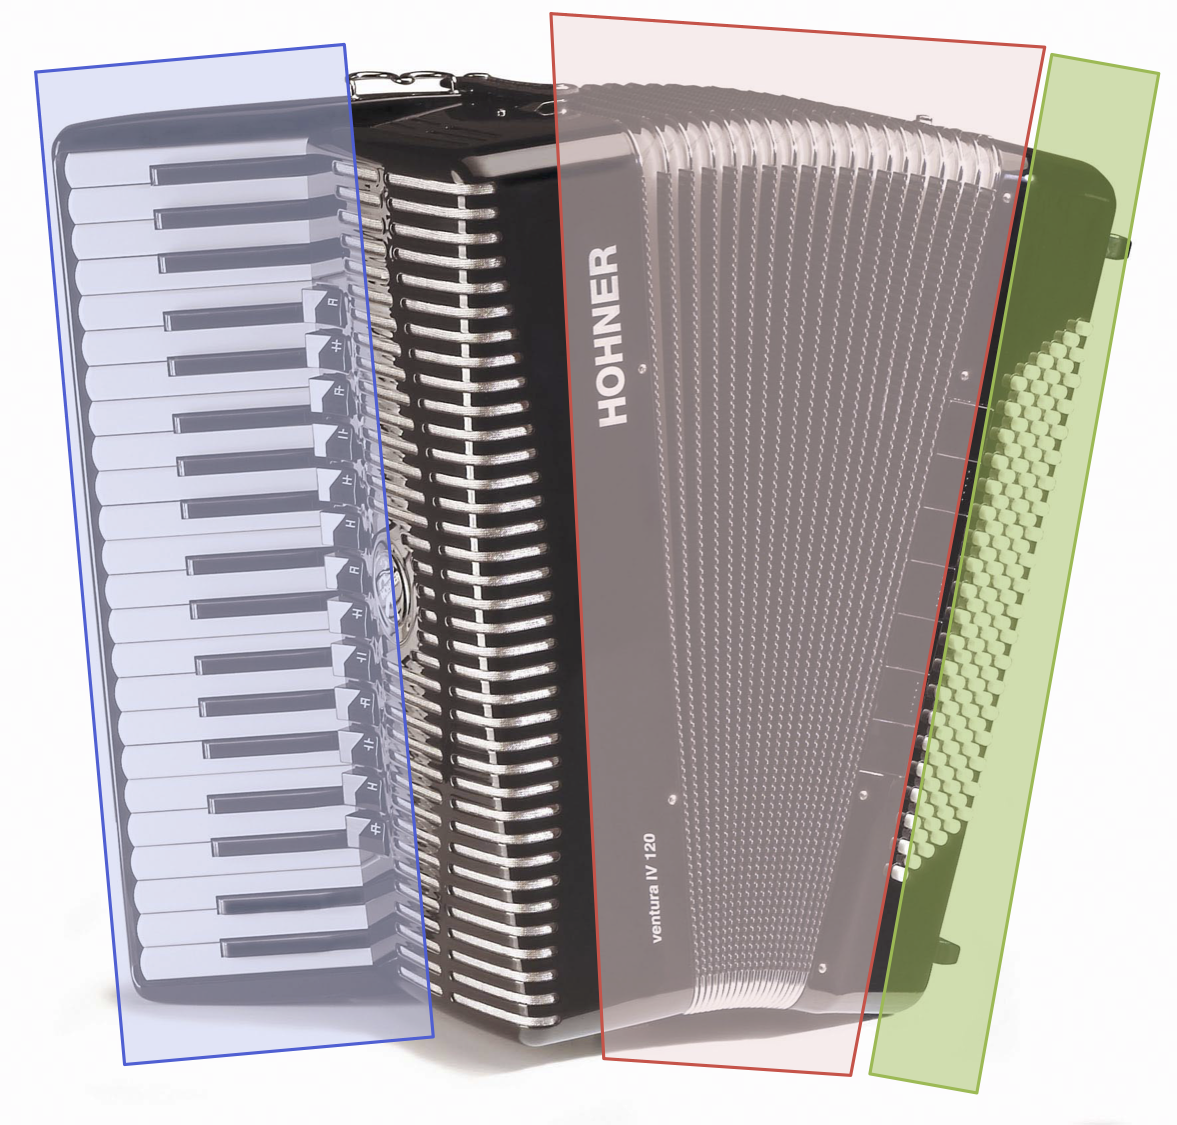
\includegraphics[width=.6\linewidth]{accordion}
	\caption{\label{fig:accordion} Humans learn new concepts (e.g., an accordion) by decomposing the concept into constituent parts (e.g., keyboard, bellows, and bass buttons) and then learning each of these parts individually.}
\end{figure}

\section{A Mathematical Model of Music Composition}
\begin{figure*}[th]
	\centering
	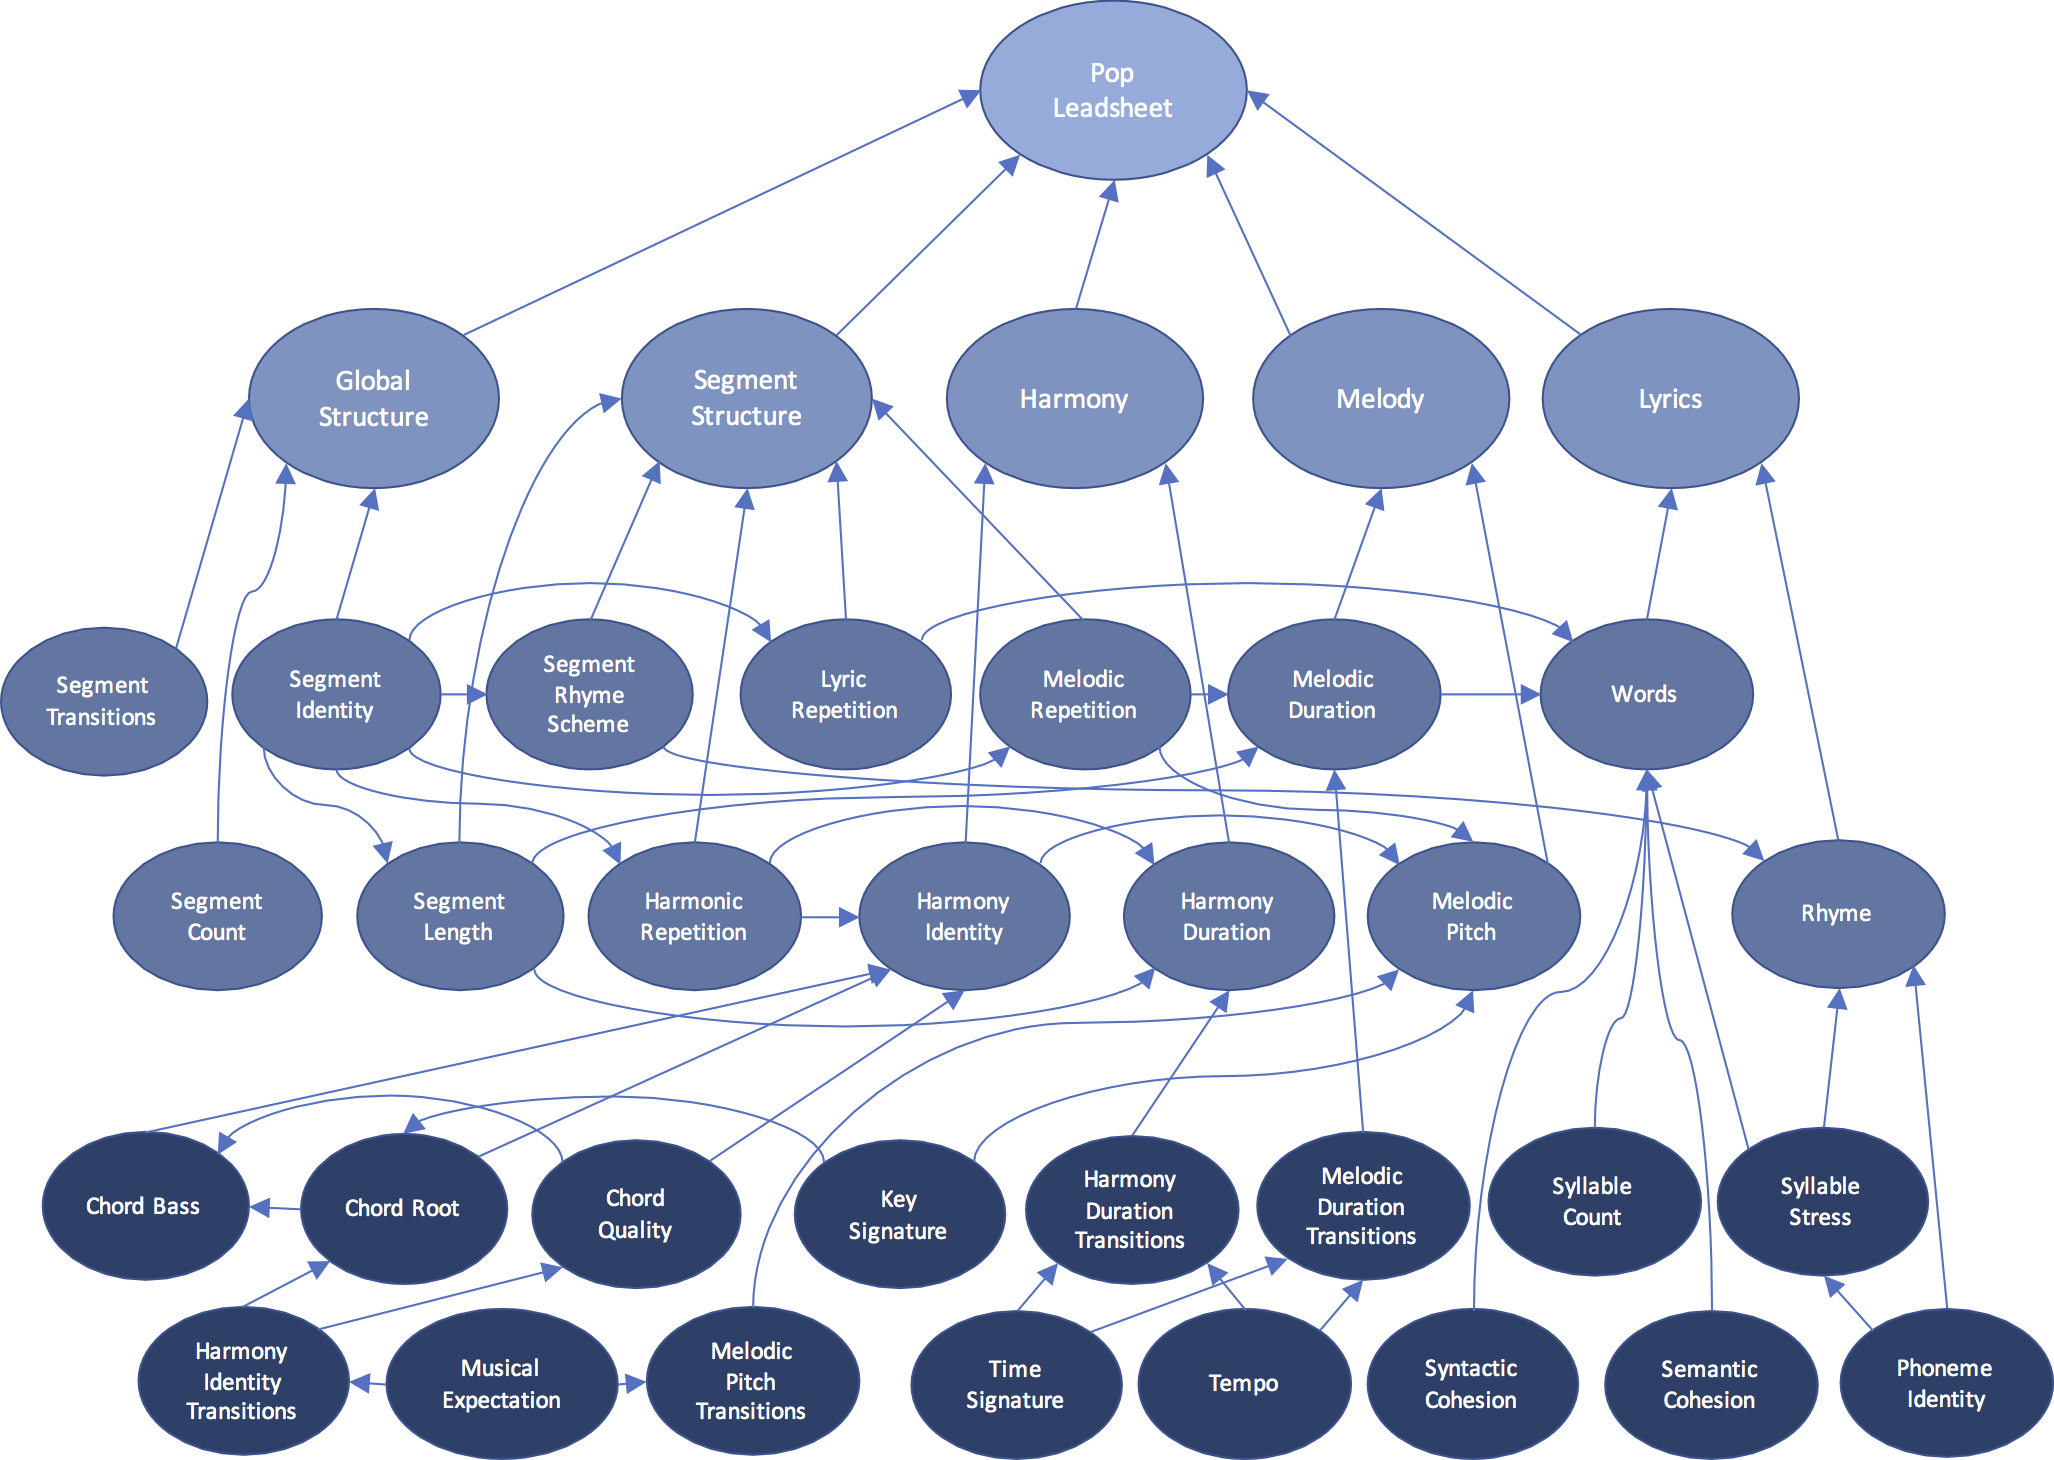
\includegraphics[width=.8\linewidth]{pop_hbpl_gradient}
	\caption{\label{fig:pop_hbpl_gradient} A graphical model of one possible HBPL model for lyrical, sectional-form music composition. Each node represents a concept or subconcept model used to define composition. The vertical layers in the graph roughly correspond to levels of domain-specificity. An arrow from a node $A$ to a node $B$ means that $B$ is conditioned on $A$.}
\end{figure*}

Patterned after the approach taken by \citeauthor{lake2015human} \shortcite{lake2015human}, we define a mathematical model of music composition using a hierarchical Bayesian program learning (HBPL) model. We define a lyrical composition as $\gamma=(\nu,\tau,\eta,\mu,\lambda)$ with intention $\nu$, structure $\tau$, harmony $\eta$, melody $\mu$, and lyrics $\lambda$. A HBPL model decomposes a composition $\gamma$, conditioned on an inspiring source $\iota$, by factoring a joint distribution over constituent variables, e.g.,

\[ P(\gamma|\iota) = P(\nu|\iota)P(\tau|\nu)P(\eta|\nu,\tau)P(\mu|\nu,\tau,\eta)P(\lambda|\nu,\tau,\mu). \] 

\noindent Each term in the factorization essentially represents a subconcept to be learned which can be further decomposed into yet simpler subconcept models. For example, we might define structure as consisting of the concepts of a global structure $\zeta$ and a section- or segment-structure $\sigma$:

\[ P(\tau|\nu) = P(\zeta|\nu)P(\sigma|\nu,\zeta) \]

At some point in this hierarchy, the subconcepts are then implemented as computational models. For example, we might implement a model of global structure $\zeta$ using a probability distribution over global structure lengths $|\zeta|$ (i.e., the number of sections in a song) and a single-order Markov model over section types (e.g., ``verse'', ``chorus'', etc.):

\[ P(\zeta|\nu) = P(|\zeta|) P(\zeta_1) \prod_{i=2}^{|\zeta|} P(\zeta_i|i,\zeta_{i-1}) \]

At each level there are many possible factorizations. Identifying which factorizations will most effectively facilitate learning is the most significant challenge to human-level concept learning in general. The classic question of ``Which comes first: the lyrics or the melody?'' suddenly evolves from anecdotal trivia to a computational design decision.

There are surely multiple viable solutions, but even articulating \emph{one} can be troublesome (see Figure~\ref{fig:pop_hbpl_gradient}). For example, we discovered that lyrics and melody have subtle interdependencies that reveal masked layers within each of these viewpoints \cite{bodily2017Mume}. This has led to more carefully defining melody and lyrics to enable effective modeling of these dependencies.


\section{Data-Driven Concept Modeling}

Given a factorization over lyrical, sectional-form compositions that effectively facilitates learning, the next challenge with human-level concept learning is how to train each of the subconcept models. In general, data-driven approaches are favorable over hand-crafted approximations inasmuch as they tend to minimize direct bias of system designers.

Choosing the right \emph{computational} model to represent a subconcept is non-trivial. Whether to use a grammar, a Markov model, or a dictionary-based approach depends both on the amount of available data and on the specific concept being modeled. We have explored several computational models for approximating subconcept models \cite{bodily2017ICCC}. Using a probability distribution over global structure lengths and a single-order Markov model over section types we might learn empirical distributions for these concepts like those shown in Figures~\ref{fig:segment_count_per_song} and~\ref{fig:segment_transitions}.

\begin{figure}
	\centering
	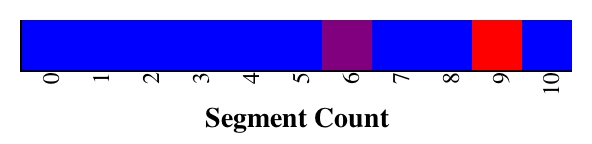
\includegraphics[width=.8\linewidth]{segment_count_per_song}
	\caption{\label{fig:segment_count_per_song} A visual representation of a possible probability distribution over the number of sections per song. Red corresponds to high probability, blue to low.}
\end{figure}

\begin{figure}[t]
	\centering
	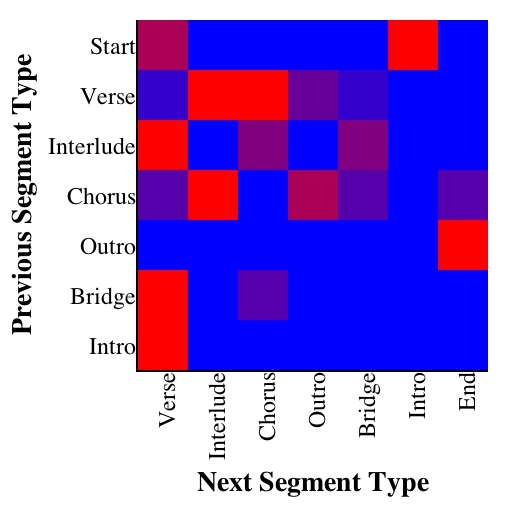
\includegraphics[width=.8\linewidth]{segment_transitions}
	\caption{\label{fig:segment_transitions} A visual representation of a possible single-order Markov transition matrix for section types. Red corresponds to high probability, blue to low. The results largely agree with intuition. For example, songs generally start with an intro and occasionally with a verse; songs generally end with an outro and occasionally a chorus; and sections of the same type do not generally follow one another.}
\end{figure}

Some concepts (e.g., global structure) are abstract in nature and are not consistently annotated in available datasets. Irrespective of the quality of these datasets, the question remains of whether abstract concepts should be explicitly modeled at all. We mention two arguments in favor of explicitly modeling. First, several attempts have been made to compose sectional-form music without explicitly modeling structure. The results of these attempts almost universally lack any notion of global structure, which represents a major flaw considering its fundamental importance in sectional-form music. The second argument for explicitly modeling global structure is that not only is it fundamental, but it strongly represents the way composers think about music and its explicit modeling is a more faithful approximation of human-level concept learning in this domain.

How then can we learn abstract concepts which are not annotated? The beauty of this question is that it shows that ``creative behaviour in people draws on a full set of intelligent abilities'' and thus how true computational creativity ``represents a serious technical challenge for Artificial Intelligence research'' \cite{colton2012computational}. Part of our research focuses on finding effective solutions to problems such as inferring global structure, key signature (for normalization), rhyme scheme, and melodic/harmonic/lyric motifs. These tasks, which human composers execute with ease, are fundamental to their ability to learn and create new music. 

We hypothesize that enabling computers with these intelligent abilities will likewise improve their ability to learn and create new music, one way being that it enables explicitly learning subconcept models of abstract concepts. We are currently investigating the use of sequence alignment over multiple viewpoints to infer global structure and rhyme scheme, both of which represent patterns of repetition and self-similarity within a composition (e.g., see Figure~\ref{fig:verse_alignment}).

\begin{figure}[t]
	\centering
	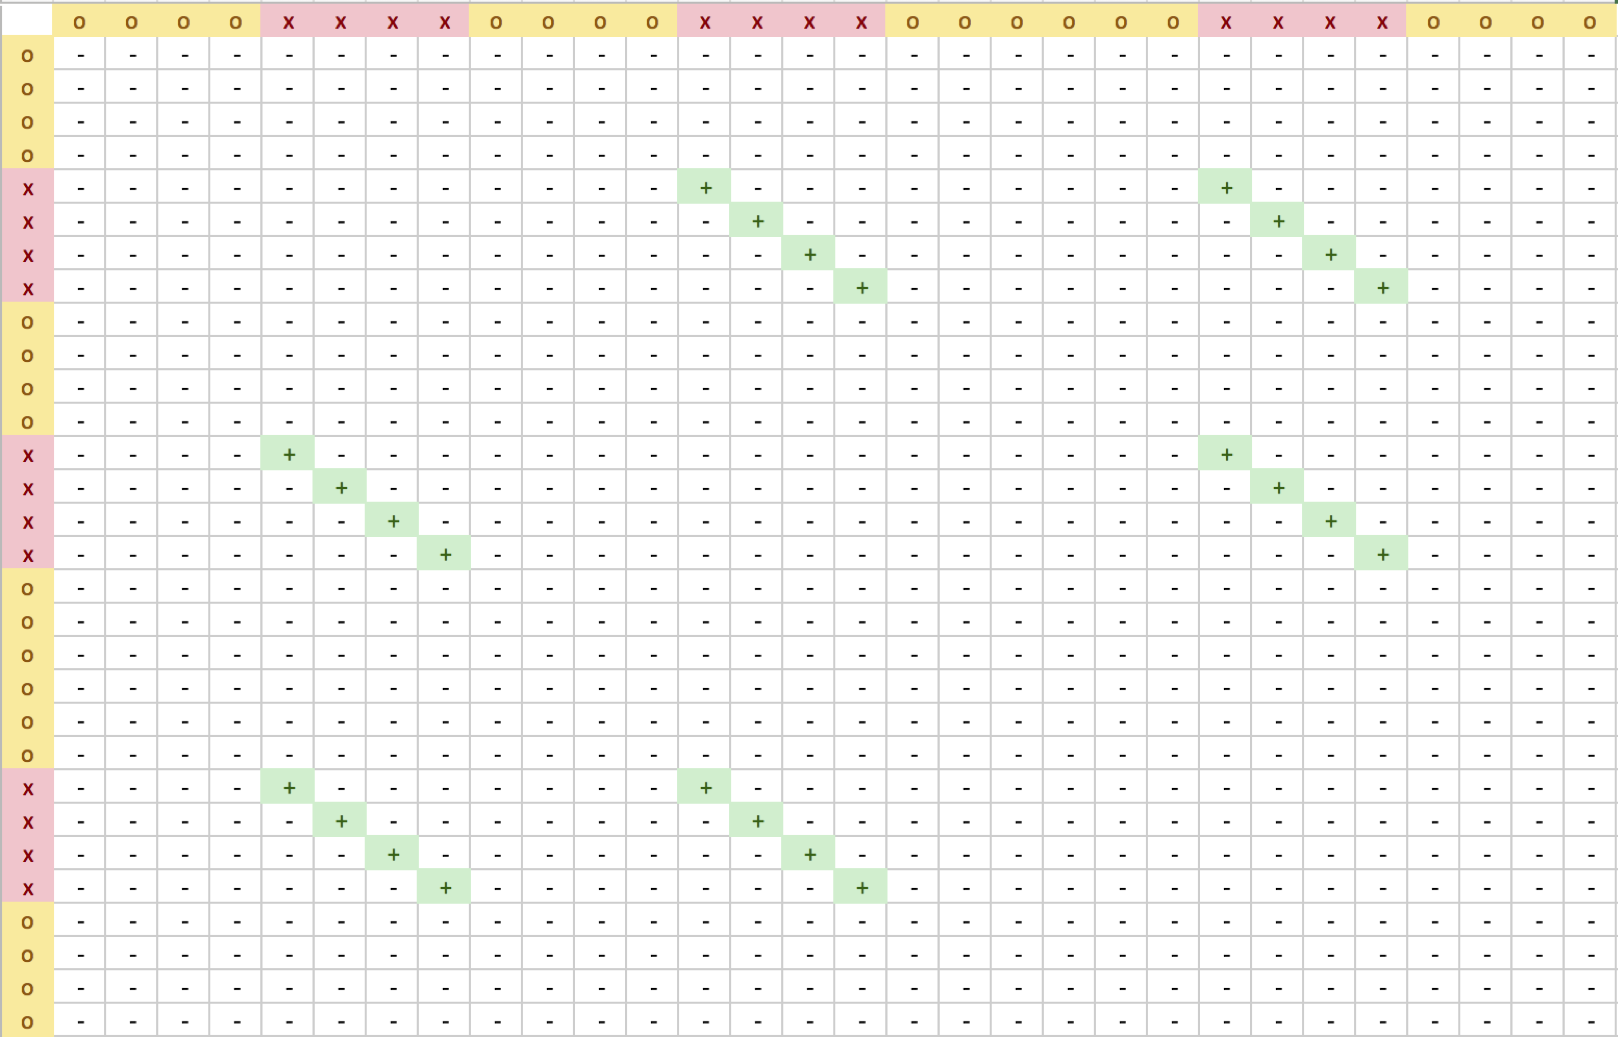
\includegraphics[width=\linewidth]{verse_alignment}
	\caption{\label{fig:verse_alignment} We can use sequence alignment algorithms over multiple viewpoints to find patterns of self-similarity within a composition representing abstract concepts such as verses, choruses, or rhyme schemes. For example, we might train scoring parameters such that a self-alignment of a composition with itself yields local similarities (shown in green) representative of verses in the composition where melody and harmony are similar, but lyrics differ (red).}
\end{figure}

\section{Intuition-Based Concept Modeling}
\begin{figure*}[t]
	\centering
	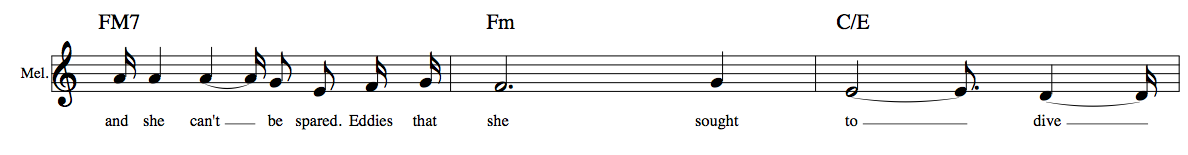
\includegraphics[width=.82\linewidth]{example}
	\caption{\label{fig:example_composition} Three measures of a sample composition generated using the HBPL framework. The full composition and others can be found online at \emph{anonymized}.}
\end{figure*}
In practice there is a dearth of lyrical, sectional-form composition data, let alone data that is completely and consistently annotated. Furthermore, at some point in the decomposition process, subconcepts become simple enough that it becomes reasonable to consider approximating concept models using intuition-based, parameterized distributions. Though manually encoding models to represent concepts limits the system according to the biases and domain-expertise of the system designer, there are several reasons to consider this approach.

First, we must realize that within the domain of lyrical, sectional-form composition, any system which successfully imitates (biases and all) even an amateur pop music artist would be deemed a success. Second, it should be noted that manually encoding subconcept models does not equate to hard-coding the output of the system. A third argument is that humans themselves often form their own mental subconcept models as a result of direct instruction from other humans rather than by learning through experience.

Human-level concept learning is by its nature already an intuition-based approach inasmuch as the primary method for factoring a model relies on the designer's intuition about the dependencies that exist between compositional viewpoints. Furthermore, as highlighted by \citeauthor{bodily2017Mume} (\citeyear{bodily2017Mume}), the modular nature of the hierarchical models allows for focused community debate and discussion, allowing designers to leverage domain-expertise and intuition from a broader community of composition artists. Thus, whereas the biases introduced from hand-crafting models might be a weakness, they might also become a strength insofar as human experts are capable of understanding subconcepts beyond how they are exhibited in any given music corpus.

As more data becomes available, hand-crafted models can easily be replaced by data-derived models. Our hypothesis is that the relative ease of hand-crafting subconcept models will at the very least serve as an effective means for testing the viability of different high-level factorizations. Using human-intuition to hand-craft parameterized subconcept models is an area of future work.

\section{Discussion}

There are several implications for a system capable of both understanding and creating novel music. A generative system of this nature could be used to compose customized music for mood therapy, video games, and personal/commercial videos. It could also be used to provide novel pop compositions for singer(-not)songwriters or aid composers in the composition process (e.g., see Figure~\ref{fig:example_composition}).

There are also several significant implications that do not involve generation. As demonstrated by \citeauthor{lake2015human} (\citeyear{lake2015human}), a HBPL model can be used to recognize abstract artefacts from concrete representations. In the domain of lyrical, sectional-form music this essentially equates to being able to automatically transcribe pop music from audio, meaning any aspiring musician could easily obtain sheet music for their favorite songs on the radio.

\citeauthor{lake2015human} (\citeyear{lake2015human}) also showed that given the ability to recognize abstract artefacts from their concrete representations, the HBPL model can also compute similarity between artefacts (e.g., for classification) based on more significant, abstract features. For music this equates to being able to effectively compare audio tracks using abstract features such as harmony, melody, and semantics in the lyrics. In an age where more music is recorded each year than could be listened to in a lifetime, music recommendation systems must incorporate this ability to enable users to quickly find music consistent with their tastes.

\section{Conclusion}

The solution to achieving creative computers is not to figure out how to remove humans from the equation; creativity is a fundamentally human endeavor insofar as it is our values and culture that in large measure define what we deem creative. The solution rather requires understanding how computers and humans must interact in order for a computer to learn to be creative. Human-level concept learning holds many clues to how machines may one day learn-to-learn creativity.

\bibliographystyle{iccc}
\bibliography{../all}


\end{document}
